\appendix
\section{Appendix}


\begin{table}[t!]
\caption{\small\textbf{Applying iBOT++ to CLIP}, on a ViT-L backbone. iBOT++ significantly enhances CLIP performance across several tasks, beyond what can be obtained with iBOT.}
\vspace{-2mm}
\scriptsize

\centering

\setlength{\tabcolsep}{3pt} 
\renewcommand{\arraystretch}{1.1} 


\resizebox{\columnwidth}{!}{
\begin{tabular}{l c c c c c c}
\small Model & Seg. & Depth $\downarrow$ & ImageNet & IT Ret. & TI Ret. & 0-shot Seg.\\
ViT-L & ADE20k & NYUv2 & KNN & COCO & COCO & PC60 \\
\midrule
CLIP & 35.7 & 0.571 & 73.5 & 52.2 & 33.2 & 4.3 \\
CLIP+iBOT & 41.3 & 0.458 & 77.2 & 55.7 & 37.5 & 8.0 \\
CLIP+iBOT++ & \textbf{42.8} & \textbf{0.434} & \textbf{78.7} & \textbf{58.1} & \textbf{40.6} & \textbf{22.9} \\
\end{tabular}
}
\label{tab:clip_full_ema}
\end{table}

\begin{table}[t!]
\caption{\small\textbf{Applying iBOT++ to CLIP with head-only EMA}, on a ViT-L backbone. iBOT++ with head-only EMA significantly enhances CLIP performance.}
\vspace{-2mm}
\scriptsize

\centering

\setlength{\tabcolsep}{3pt} 
\renewcommand{\arraystretch}{1.1} 


\resizebox{\columnwidth}{!}{
\begin{tabular}{l c c c c c c}
\small Model & Seg. & Depth $\downarrow$ & ImageNet & IT Ret. & TI Ret. & 0-shot Seg.\\
ViT-L & ADE20k & NYUv2 & KNN & COCO & COCO & PC60 \\
\midrule
CLIP & 35.7 & 0.571 & 73.5 & 52.2 & 33.2 & 4.3 \\
CLIP+iBOT & 39.8 & 0.467 & 76.6 & 55.4 & 37.0 & 4.3 \\
CLIP+iBOT++ & \textbf{42.5} & \textbf{0.437} & \textbf{78.2} & \textbf{56.6} & \textbf{39.3} & \textbf{22.1} \\
\end{tabular}
}
\label{tab:clip}
\end{table}

\begin{table}[t!]
\caption{\small\textbf{Applying iBOT++ to CLIP with a dual CLS setup}, on a ViT-g backbone. iBOT++ significantly enhances performance across several tasks, beyond what can be obtained with iBOT.}
\vspace{-2mm}
\scriptsize

\centering

\setlength{\tabcolsep}{3pt} 
\renewcommand{\arraystretch}{1.1} 


\resizebox{\columnwidth}{!}{
\begin{tabular}{l c c c c c c}
\small Model & Seg. & Depth $\downarrow$ & ImageNet & IT Ret. & TI Ret. & 0-shot Seg.\\
ViT-g & ADE20k & NYUv2 & KNN & COCO & COCO & PC60 \\
\midrule
CLIP 2 CLS & 40.1 & 0.475 & 79.1 & 72.9 & 56.1 & 18.2 \\
CLIP 2 CLS + iBOT & 41.1 & 0.442 & 81.6 & 73.2 & 58.3 & 16.4 \\
CLIP 2 CLS + iBOT++ & \textbf{47.2} & \textbf{0.366} & \textbf{82.7} & \textbf{73.6} & \textbf{58.9} & \textbf{28.2} \\
\end{tabular}
}
\label{tab:clip_dual}
\end{table}



\subsection{Applying iBOT++ to CLIP}


In the main paper results, we showed the value of our novel iBOT++ loss in the context of the TIPS training recipe.
In this section, we go further to demonstrate the generalizability of iBOT++ to other vision-language architectures, specifically on top of the widely adopted CLIP model.
First, both iBOT and iBOT++ are applied on top of vanilla CLIP, trained with the same dataset used throughout the paper, using a ViT-L backbone.
Our results in \cref{tab:clip_full_ema} demonstrate that integrating iBOT++ yields consistent performance gains across all metrics, beyond that of adding iBOT alone.
A similar conclusion is obtained when using head-only EMA in addition to iBOT++, a setup which reduces memory requirements significantly and achieves generally on par performance with the full EMA case, as reported in \cref{tab:clip}.
Then, as an additional experiment to validate iBOT++, we add it on top of CLIP using two CLS tokens (as in the TIPS setup, but without any of the additional losses used in TIPS), with a ViT-g backbone and the same training dataset (\cref{tab:clip_dual}).
Once again, we see significant and consistent performance gains using iBOT++, compared to the CLIP 2 CLS baseline and its modified version using iBOT.
Notably, in all these cases iBOT++ yields significant improvements in zero-shot segmentation, highlighting its importance for aligning image patches to language.
These results corroborate the usefulness of our proposed iBOT++ recipe for vision-language pretraining.

\subsection{iBOT++ Ablation Study on Masking Ratios}

\begin{table}[t!]


\caption{\small \textbf{Masking ablation for iBOT++ pretraining.} We conduct an ablation study on TIPS~\citep{tips_paper} ViT-L models to determine the optimal masking ratio for iBOT++ pretraining. 
The results show that $75\%$ masking ratio is critical for achieving strong performance across all evaluations, particularly enhancing patch-text alignment.
The model achieving the best overall performance is highlighted.}
\vspace{-2mm}
\scriptsize
\setlength{\tabcolsep}{4pt} %
\centering
{
\begin{tabular}{c c c c c c c c}
\small Masking & Segmentation $\uparrow$ & Depth $\downarrow$ & I$\rightarrow$T Ret. $\uparrow$ &  Zero-shot Seg. $\uparrow$ \\
Ratio & PASCAL & NYUv2 & Flickr & ADE150 \\
\midrule
0.0 & 78.8 & 0.513 & 90.0 & 1.0 \\
0.5 & 82.5 & 0.438 & 92.6  & 2.4 \\
0.75 & \textbf{82.6} & \textbf{0.418} & \textbf{93.8} & \textbf{13.6} \\
\end{tabular}
}
\label{tab:masking}
\end{table}


As detailed in \cref{bridge}, distillation significantly enhances patch-text alignment, even when the teacher model exhibits poor dense alignment.
In \cref{tab:init}, we identified two key distinctions between the distillation and pretraining stages: A) also applying loss to visible tokens (compare rows (1-2)) and B) lowering masking ratio from  $75\% \rightarrow 0\%$ (compare rows (2-4)) .
In iBOT++, we propose to take the approach in A) from distillation and apply it to pretraining. 
This naturally raises the question: Would applying B) by removing masking in iBOT++ pretraining also further enhance patch-text alignment?
To explore this, we ablated the masking ratio during iBOT++ pretraining. 
Our experiments in \cref{tab:masking} demonstrate that the answer is no: iBOT++ achieves its best performance with a $75\%$ masking ratio.
As a result, we adopt the $75\%$ ratio setting as our final \tipsvtwo training recipe.
Our results confirm that Masked Image Modeling (MIM) remains critical for pretraining, consistently improving performance across image-only tasks and image-text tasks. We conclude that mask removal is only effective during distillation because the teacher model already provides the necessary strong local semantic understanding. This allows the student vision encoder to inherit the alignment without needing to learn it via the MIM objective.

\subsection{Ablations on Multi-Granularity Captions}

In \cref{tab:multi_captions}, we present ablations to justify our strategy to utilize multiple captions, varying 1-2 [CLS] tokens and the assignment to [CLS] tokens between the 3 available captions (web, PaliGemma, Gemini).
These ablations are conducted with the default \tipsvtwo training setup, except that full EMA is used (instead of head-only EMA).
We find the optimal strategy is the recipe in \tipsvtwo: alternating real/synthetic captions with the dual CLS setup.

\begin{table}[t!]
\caption{\small\textbf{Ablations for multi-granularity captions}, on ViT-g. Texts for 2 CLS are separated by \textbf{/} and for each CLS, texts are uniformly sampled from sources. }
\vspace{-3mm}
\centering
\setlength{\tabcolsep}{3pt} 
\renewcommand{\arraystretch}{1.1} 

\resizebox{\columnwidth}{!}{
\begin{tabular}{l c c c c c c}
\multirow{2}{*}{Text Strategy} & Seg. & Depth $\downarrow$ & ImageNet & IT Ret. & 0-shot Seg.  \\
& ADE20k & NYUv2 & KNN & COCO & ADE150 \\
\midrule

1 CLS (web, PaliGemma) & 46.3 & 0.375 & 80.4 & 72.3 & 16.4 \\
1 CLS (web, PaliGemma, Gemini) & 46.7 & 0.366 & 81.2 & 74.4 & 17.7 \\
2 CLS (web / PaliGemma) & 48.3 & 0.370 & \textbf{84.3} & 70.0 & 17.1 \\
2 CLS (web / PaliGemma, Gemini) & \textbf{49.1} & \textbf{0.354} & \textbf{84.3} & 
\textbf{76.2} & \textbf{18.1} \\


\end{tabular}
}
\label{tab:multi_captions}
\end{table}


\subsection{Qualitative Comparisons to DINOv2 and v3}

In order to further illustrate the comparison with self-supervised pretrained models, we provide additional PCA maps for DINOv2 (with registers)~\cite{vitsneedregisters,oquab2024dinov2} and DINOv3~\citep{siméoni2025dinov3}.
\cref{fig:qualitative_dino_l} presents results on ViT-L models, which is the largest common size between these model families. 
\cref{fig:qualitative_dino_g} presents results on larger models: ViT-g for DINOv2 and \tipsvtwo, but ViT-7B for DINOv3.
Note that the DINOv3 ViT-7B teacher model is trained with 6$\times$ more parameters and 15$\times$ more images than the \tipsvtwo ViT-g teacher.

Comparing DINOv3 and \tipsvtwo, we can see that PCA maps for DINOv3 are smoother, whereas \tipsvtwo maps are more granular.
We note that DINOv3 enhances dense feature maps (on top of DINOv2) by means of a Gram anchoring loss that acts on patch correlations, introducing another teacher that is frozen from the past, along with a higher-resolution inference and down-sampling procedure.
The dense feature maps of \tipsvtwo also demonstrate comparable improvements in spatial coherence (on top of TIPS), but require much simpler changes to the training setup.
On some images, this seems to demonstrate a more semantic focus for \tipsvtwo, compared to a more spatial focus in DINOv3.

For example, in the third row of \cref{fig:qualitative_dino_l} and \cref{fig:qualitative_dino_g}, the backpacks appear semantically similar to the people wearing them in DINOv3 PCA, while they are clearly distinct from the people in \tipsvtwo PCA.
In the second row of \cref{fig:qualitative_dino_g}, the ceiling tends to be underclustered in DINOv3, unable to distinguish lamps and other features; in contrast, \tipsvtwo clearly segments them properly.
In the first row of \cref{fig:qualitative_dino_l}, the windows for DINOv3 PCA are distinctly colored, varying from foreground to background, but are all uniformly colored for \tipsvtwo PCA.

Comparing against DINOv2, \tipsvtwo PCA maps are overall much smoother and more spatially coherent, in contrast to DINOv2's noisy maps.




\newcommand{\showpcas}[2]{%
  \resizebox{#1\linewidth}{!}{%
	\setlength{\fboxsep}{0pt}
		\hfill
		\includegraphics[height=#1\linewidth]{images/supp/#2.jpeg}
		\hfill
		\includegraphics[height=#1\linewidth]{images/supp/dinov2/vit_l/#2.png}
		\hfill
        \includegraphics[height=#1\linewidth]{images/supp/dinov3/vit_l/#2.png}
		\hfill
		\includegraphics[height=#1\linewidth]{images/supp/tipsv2/vit_l/#2.png}
}}

\newcommand{\pcawidthsupp}{1.0}

\begin{figure}[tb]
	\centering
	\showpcas{\pcawidthsupp}{dadaocheng} \\[0.2mm]
    \showpcas{\pcawidthsupp}{cph} \\[0.2mm]
    \showpcas{\pcawidthsupp}{hike} \\[0.2mm]
    \showpcas{\pcawidthsupp}{angus} \\[0.1mm]

    \resizebox{\pcawidthsupp\linewidth}{!}{%
    \scriptsize
        \begin{minipage}[t]{0.24\linewidth}
          \centering
          Image
        \end{minipage}%
        \hfill
        \begin{minipage}[t]{0.24\linewidth}
          \centering
          DINOv2-L
        \end{minipage}%
        \hfill
        \begin{minipage}[t]{0.24\linewidth}
          \centering
          DINOv3-L
        \end{minipage}%
        \hfill
        \begin{minipage}[t]{0.24\linewidth}
          \centering
          \tipsvtwo-L (ours)
        \end{minipage}%
    }%
    \vspace{-1mm}
	\caption{\small\textbf{PCA maps at ViT-L size.} Comparing the first $3$ PCA components from the ViT-L models of DINOv2 (with registers), DINOv3, and \tipsvtwo. Images are forwarded at $1372$ resolution for patch size $14$ models (DINOv2 and \tipsvtwo) and at $1568$ resolution for patch size $16$ models (DINOv3). DINOv3 features appear smoother, but \tipsvtwo features show more semantically focused features, e.g., \tipsvtwo maps show all windows clustered together in row 1, and the eyes and leash are distinct on the dog in row 4.}
	\label{fig:qualitative_dino_l}
	\vspace{-3mm}
\end{figure}

\newcommand{\showpcasg}[2]{%
  \resizebox{#1\linewidth}{!}{%
	\setlength{\fboxsep}{0pt}
		\hfill
		\includegraphics[height=#1\linewidth]{images/supp/#2.jpeg}
		\hfill
		\includegraphics[height=#1\linewidth]{images/supp/dinov2/vit_g/#2.png}
		\hfill
        \includegraphics[height=#1\linewidth]{images/supp/dinov3/vit_7b/#2.png}
		\hfill
		\includegraphics[height=#1\linewidth]{images/supp/tipsv2/vit_g/#2.png}
}}

\begin{figure}[tb]
	\centering
	\showpcasg{\pcawidthsupp}{dadaocheng} \\[0.2mm]
    \showpcasg{\pcawidthsupp}{cph} \\[0.2mm]
    \showpcasg{\pcawidthsupp}{hike} \\[0.2mm]
    \showpcasg{\pcawidthsupp}{angus} \\[0.1mm]

    \resizebox{\pcawidthsupp\linewidth}{!}{%
    \scriptsize
        \begin{minipage}[t]{0.24\linewidth}
          \centering
          Image
        \end{minipage}%
        \hfill
        \begin{minipage}[t]{0.24\linewidth}
          \centering
          DINOv2-g
        \end{minipage}%
        \hfill
        \begin{minipage}[t]{0.24\linewidth}
          \centering
          DINOv3-7B
        \end{minipage}%
        \hfill
        \begin{minipage}[t]{0.24\linewidth}
          \centering
          \tipsvtwo-g (ours)
        \end{minipage}%
    }%
    \vspace{-1mm}
	\caption{\small\textbf{PCA maps at ViT-g or ViT-7B size.} Comparing the first $3$ PCA components from teacher models of DINOv2  (with registers, ViT-g), DINOv3 (ViT-7B), and \tipsvtwo (ViT-g). Images are forwarded at $1372$ resolution for patch size $14$ models (DINOv2 and \tipsvtwo) and at $1568$ resolution for patch size $16$ models (DINOv3). 
    As for the ViT-L PCA maps, DINOv3 features appear smoother, but \tipsvtwo features capture more semantically focused details, e.g., notice the ceiling details in row 2 or the different colors contrasting people and backpacks in row 3.}
	\label{fig:qualitative_dino_g}
	\vspace{-3mm}
\end{figure}



\subsection{Qualitative Analysis: iBOT++ vs iBOT}

\newcommand{\showvizs}[2]{%
  \resizebox{#1\linewidth}{!}{%
	\setlength{\fboxsep}{0pt}
		\includegraphics[height=#1\linewidth]{images/supp/#2.png}
		\hfill
		\includegraphics[height=#1\linewidth]{images/supp/#2_gt.png}
		\hfill
		\includegraphics[height=#1\linewidth]{images/supp/#2_ibotplus.png}
		\hfill
		\includegraphics[height=#1\linewidth]{images/supp/#2_ibot.png}
}}


\newcommand{\vizwidthsupp}{1.0}
\begin{figure}[tb]
	\centering
	\showvizs{\vizwidthsupp}{bicycle} \\[0.24mm]
    \showvizs{\vizwidthsupp}{kids} \\[0.24mm]
    \showvizs{\vizwidthsupp}{baby} \\[0.24mm]
    \showvizs{\vizwidthsupp}{redbus} \\[0.24mm]
    \showvizs{\vizwidthsupp}{puppy} \\[0.24mm]
    \showvizs{\vizwidthsupp}{sleep} \\[0.24mm]

    \resizebox{\vizwidthsupp\linewidth}{!}{%
    \scriptsize
        \begin{minipage}[t]{0.24\linewidth}
          \centering
          Image
        \end{minipage}%
        \hfill
        \begin{minipage}[t]{0.24\linewidth}
          \centering
          Ground truth
        \end{minipage}%
        \hfill
        \begin{minipage}[t]{0.24\linewidth}
          \centering
          iBOT++
        \end{minipage}%
        \hfill
        \begin{minipage}[t]{0.24\linewidth}
          \centering
          iBOT
        \end{minipage}%
    }%
    \vspace{-1mm}
	\caption{\small\textbf{Zero-shot segmentation visualization.} Comparing results with the iBOT loss (used in TIPS) vs the iBOT++ loss (used in \tipsvtwo), where classes are predicted directly by finding the closest text embedding to each image patch token, without any post-processing. Compared to baseline iBOT, iBOT++ achieves significantly improved patch-text alignment, as part of the TIPSv2 recipe.}
	\label{fig:ibotplus_zss_viz}
	\vspace{-3mm}
\end{figure}

As detailed in \cref{loss_diff}, iBOT++ significantly enhances patch-text alignment during pretraining.
This improvement is quantified in \cref{tab:ablation_studies}, where a substantial performance gain is directly observed in the zero-shot segmentation metrics when comparing iBOT baseline (first row) to iBOT++ (second row). 
To further illustrate this enhancement, \cref{fig:ibotplus_zss_viz} provides qualitative visualizations of the zero-shot segmentation results, which correspond directly to the first and second rows of \cref{tab:ablation_studies}. These visualizations confirm that iBOT++ yields significantly cleaner segmentation maps.

\subsection{Zero-shot Segmentation with SigLIP2}

We showed that smaller models in the TIPS~\cite{tips_paper} family outperform larger ones in the task of zero-shot image segmentation, which motivated our investigations and contributions towards TIPSv2.
In this section, we provide evidence of a similar effect also happening in the SigLIP2 family.
\cref{tab:zeroseg_scale_siglipv2} presents zero-shot segmentation results for three model sizes, where the smallest one outperforms the larger versions in two evaluations, and the SO size model wins in the third; notably, the largest ViT-g model presents the worst performance in all three evaluations.
Note that the smallest ViT-B size model is distilled via active data curation from a larger SO model in the family.
Similarly to the TIPS case, these results indicate that the smaller models surprisingly outperform larger pretrained ones.

\begin{table}[t]
\caption{\small\textbf{Zero-shot segmentation for SigLIP2 models.} Similarly to TIPS, the smaller models tend to outperform larger ones in the same model family.}
\vspace{-2mm}
\scriptsize
\centering
{
\begin{tabular}{l c c c}
\small \multirow{2}{*}{Model} & \multicolumn{3}{c}{Zero-shot Segmentation (mIoU) $\uparrow$} \\
 & PC60 & VOC21 & ADE150 \\
\midrule
SigLIP2 B/16 & \bf{22.6} & 25.8 & \bf{16.4} \\
SigLIP2 SO/14 & 19.6 & \bf{26.8} & 15.6 \\
SigLIP2 g/16 & 17.2 & 25.7 & 13.9 \\
\end{tabular}
}
\vspace{-0mm}
\label{tab:zeroseg_scale_siglipv2}
\end{table}

\begin{table*}[t]
\caption{\small \textbf{Evaluations for all \tipsvtwo model variants.} We report four distinct \tipsvtwo model sizes (ViT-B, ViT-L, ViT-g, and SO-400m). Only the ViT-g model is pretrained; the other sizes (ViT-B, ViT-L, and SO-400m) are distilled from the ViT-g teacher. Best performance for each task is highlighted.}
\vspace{-2mm}
\scriptsize
\addtolength{\tabcolsep}{0.5em}
\centering
{
\begin{tabular}{l c c c c c c c}
\small \multirow{2}{*}{Model} & Segmentation $\uparrow$ & Depth $\downarrow$ & Normals $\downarrow$ & KNN $\uparrow$ & I$\rightarrow$T Ret. $\uparrow$ & T$\rightarrow$I Ret. $\uparrow$ & Zero-shot Seg. $\uparrow$ \\
& PASCAL & NYUv2 & NYUv2 & ImageNet & Flickr & Flickr & ADE150 \\
\midrule
\tipsvtwo B/14 & 84.0 & 0.374 & 23.2 & 79.8 & 92.6 & 80.0 & 17.4 \\
\tipsvtwo L/14 & 85.1 & 0.339 & 21.9 & 82.5 & \textbf{95.4} & 83.3 & \textbf{24.7} \\
\tipsvtwo SO/14 & \textbf{85.2} & 0.339 & \textbf{21.7} & 82.8 & 94.8 & 84.0 & 23.3 \\
\tipsvtwo g/14 & 85.1 & \textbf{0.334} & \textbf{21.7} & \textbf{83.7} & 95.1 & \textbf{85.9} & 17.8 \\
\end{tabular}
}
\label{tab:family}
\end{table*}


\subsection{\textbf{\tipsvtwo} Family} 
\label{sec:panda_family}



The \tipsvtwo model family includes variants with different backbone sizes: ViT-B, ViT-L, ViT-g and SO-400m~\citep{alabdulmohsin2023sovit} (referred to as $\text{SO}$ hereafter). The ViT-g model is directly pretrained, while the smaller ViT-B, ViT-L, and $\text{SO}$ variants are obtained via the patch-level distillation strategy detailed in \cref{sec:preliminaries} and \cref{bridge}, using $\text{ViT}$-g as the teacher model. For text encoder scaling, we follow \citep{tips_paper} and adopt the same transformer parameterization as the image encoder but fix the number of layers at 12 (except for the $\text{SO}$ variant, which maintains its standard layer count). 

Our studies demonstrate that the \tipsvtwo family exhibits strong performance across all image and image-text benchmarks, as summarized in \cref{tab:family}. The parameter count for each model is detailed in \cref{tab:num_params}.

\begin{table}[t]
\scriptsize
\caption{\small\textbf{Number of parameters for all \tipsvtwo model variants.} We release $4$ different model variants. For B, L and g model sizes, we use a fixed number of 12 layers in the text encoder; for the SO size, we use the same number of layers in both the image and text encoders.
}
\addtolength{\tabcolsep}{0.5em}
\centering
{
\begin{tabular}{l c c c}
Model & Image \# Params & Text \# Params &  Total \# Params \\
\midrule
\tipsvtwo-B/14 & 86.3M & 109.6M & 195.9M \\
 \tipsvtwo-L/14 & 304.0M & 183.9M & 487.9M  \\
 \tipsvtwo-SO/14 & 413.3M & 448.3M & 861.7M  \\
 \tipsvtwo-g/14 & 1.1B & 389.1M & 1.5B \\
\end{tabular}
}
\label{tab:num_params}
\end{table}




\subsection{Performance of \tipsvtwo against Competitors}

\begin{figure}[t]
    \centering
    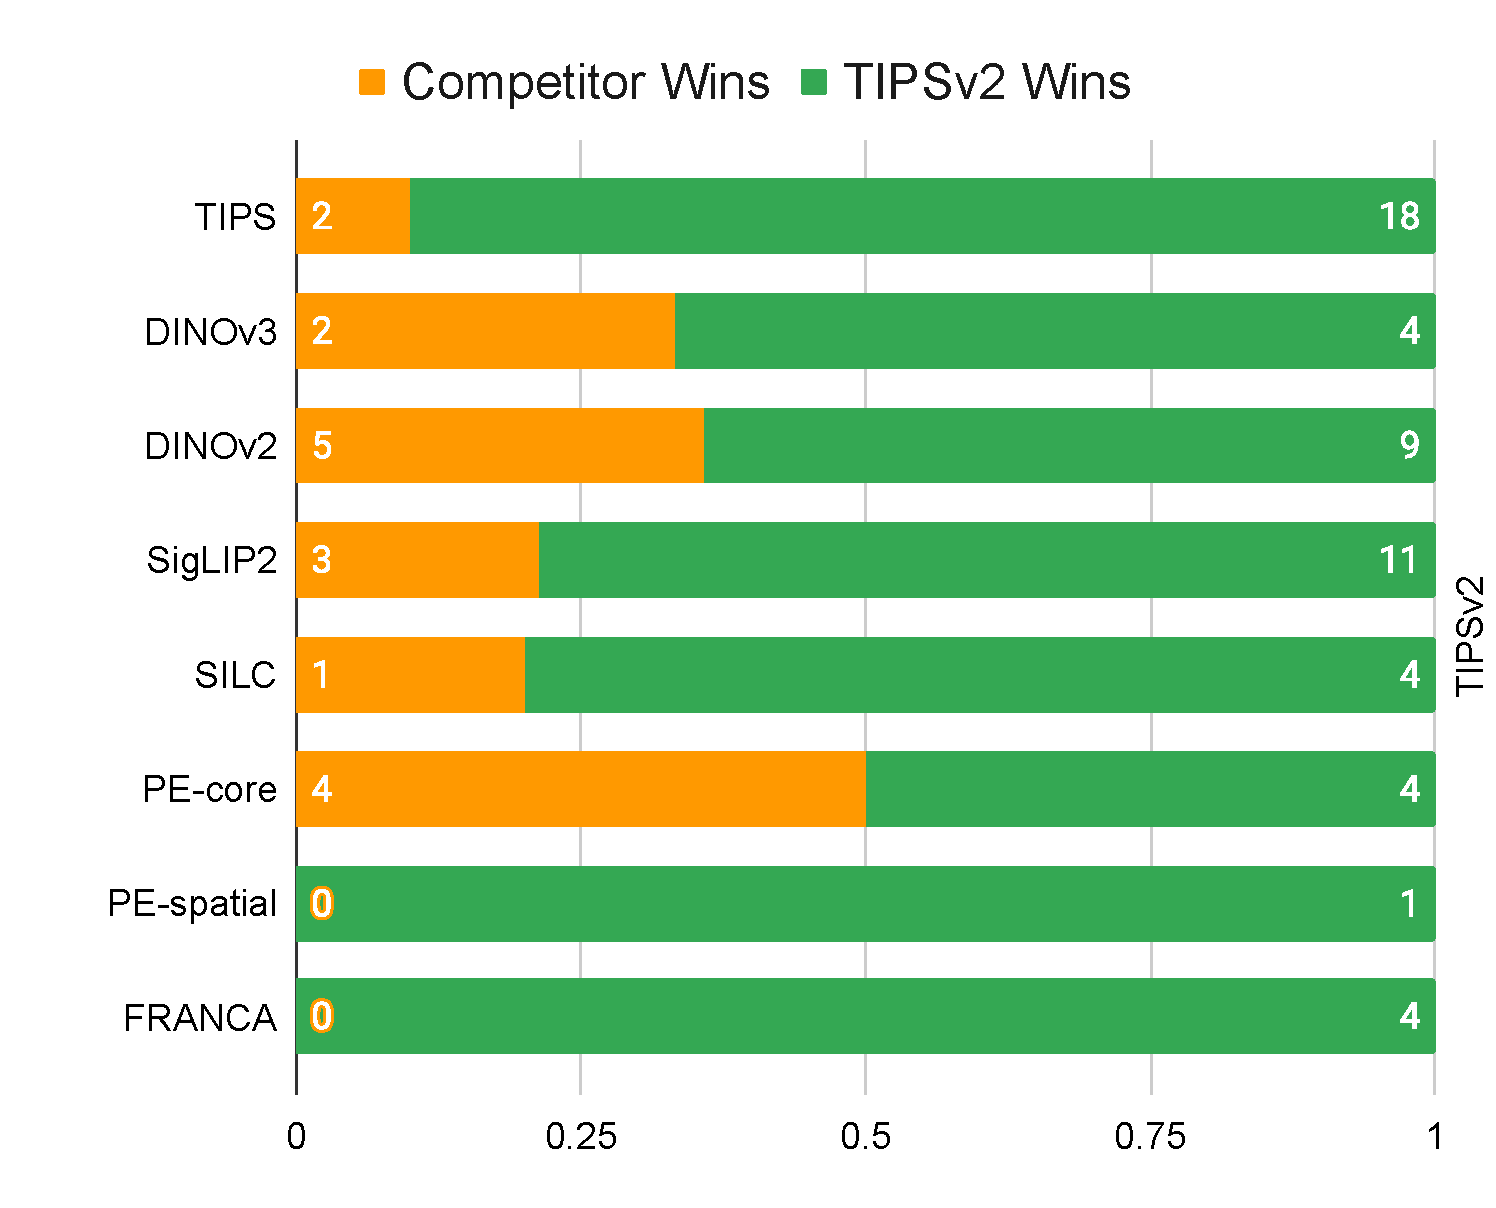
\includegraphics[width=1.0\linewidth]{figures/tipsv2-battle-fix.pdf}
    \caption{    
    \textbf{Comparison of \tipsvtwo against recent vision encoders.} The chart illustrates the percentage of shared evaluation benchmarks where \tipsvtwo secures the best result (green) compared head-to-head to other individual leading models (orange). 
    \tipsvtwo demonstrates a winning record on the majority of shared tasks. The integer displayed on the chart represents the count of metrics on which each respective model achieves the best result (i.e., the number of wins).
    For each comparison between individual vision encoders, we use the largest comparable model size (ViT-g against ViT-g, or ViT-g against ViT-G, or ViT-L against ViT-L).
    }
    \label{fig:battle}
\end{figure}

To gain a comprehensive understanding of the performance of our new method compared to other recent vision encoders, we quantified the number of evaluations where \tipsvtwo outperforms (or underperforms) each competitor method head-to-head, based on reported scores in the main results tables.
Looking only at the evaluations the models share, \tipsvtwo generally comes out on top in most cases, as shown in \cref{fig:battle}.
This summary confirms the strong results from \tipsvtwo overall.






\subsection{Additional Implementation Details}
 Our implementation closely follows that of TIPS. The loss components are weighted by $\mathcal{L} = \mathcal{L}_\text{CLIP} + \alpha\mathcal{L}_\text{DINO} + \beta\mathcal{L}_\text{iBOT}$, where $\alpha=1.0$, $\beta=2.0$. $\mathcal{L}_\text{CLIP}$ is the averaged result of contrastive losses from the two captions. We use the Adafactor~\citep{shazeer2018adafactor} optimizer, and projection heads are balanced from collapse with EMA centering and sharpening.
